\section{Periodiska systemet}
\vfill
\begin{figure}[h!]
    \centering
    \label{fig:periodic-table}
    \makebox[\textwidth]{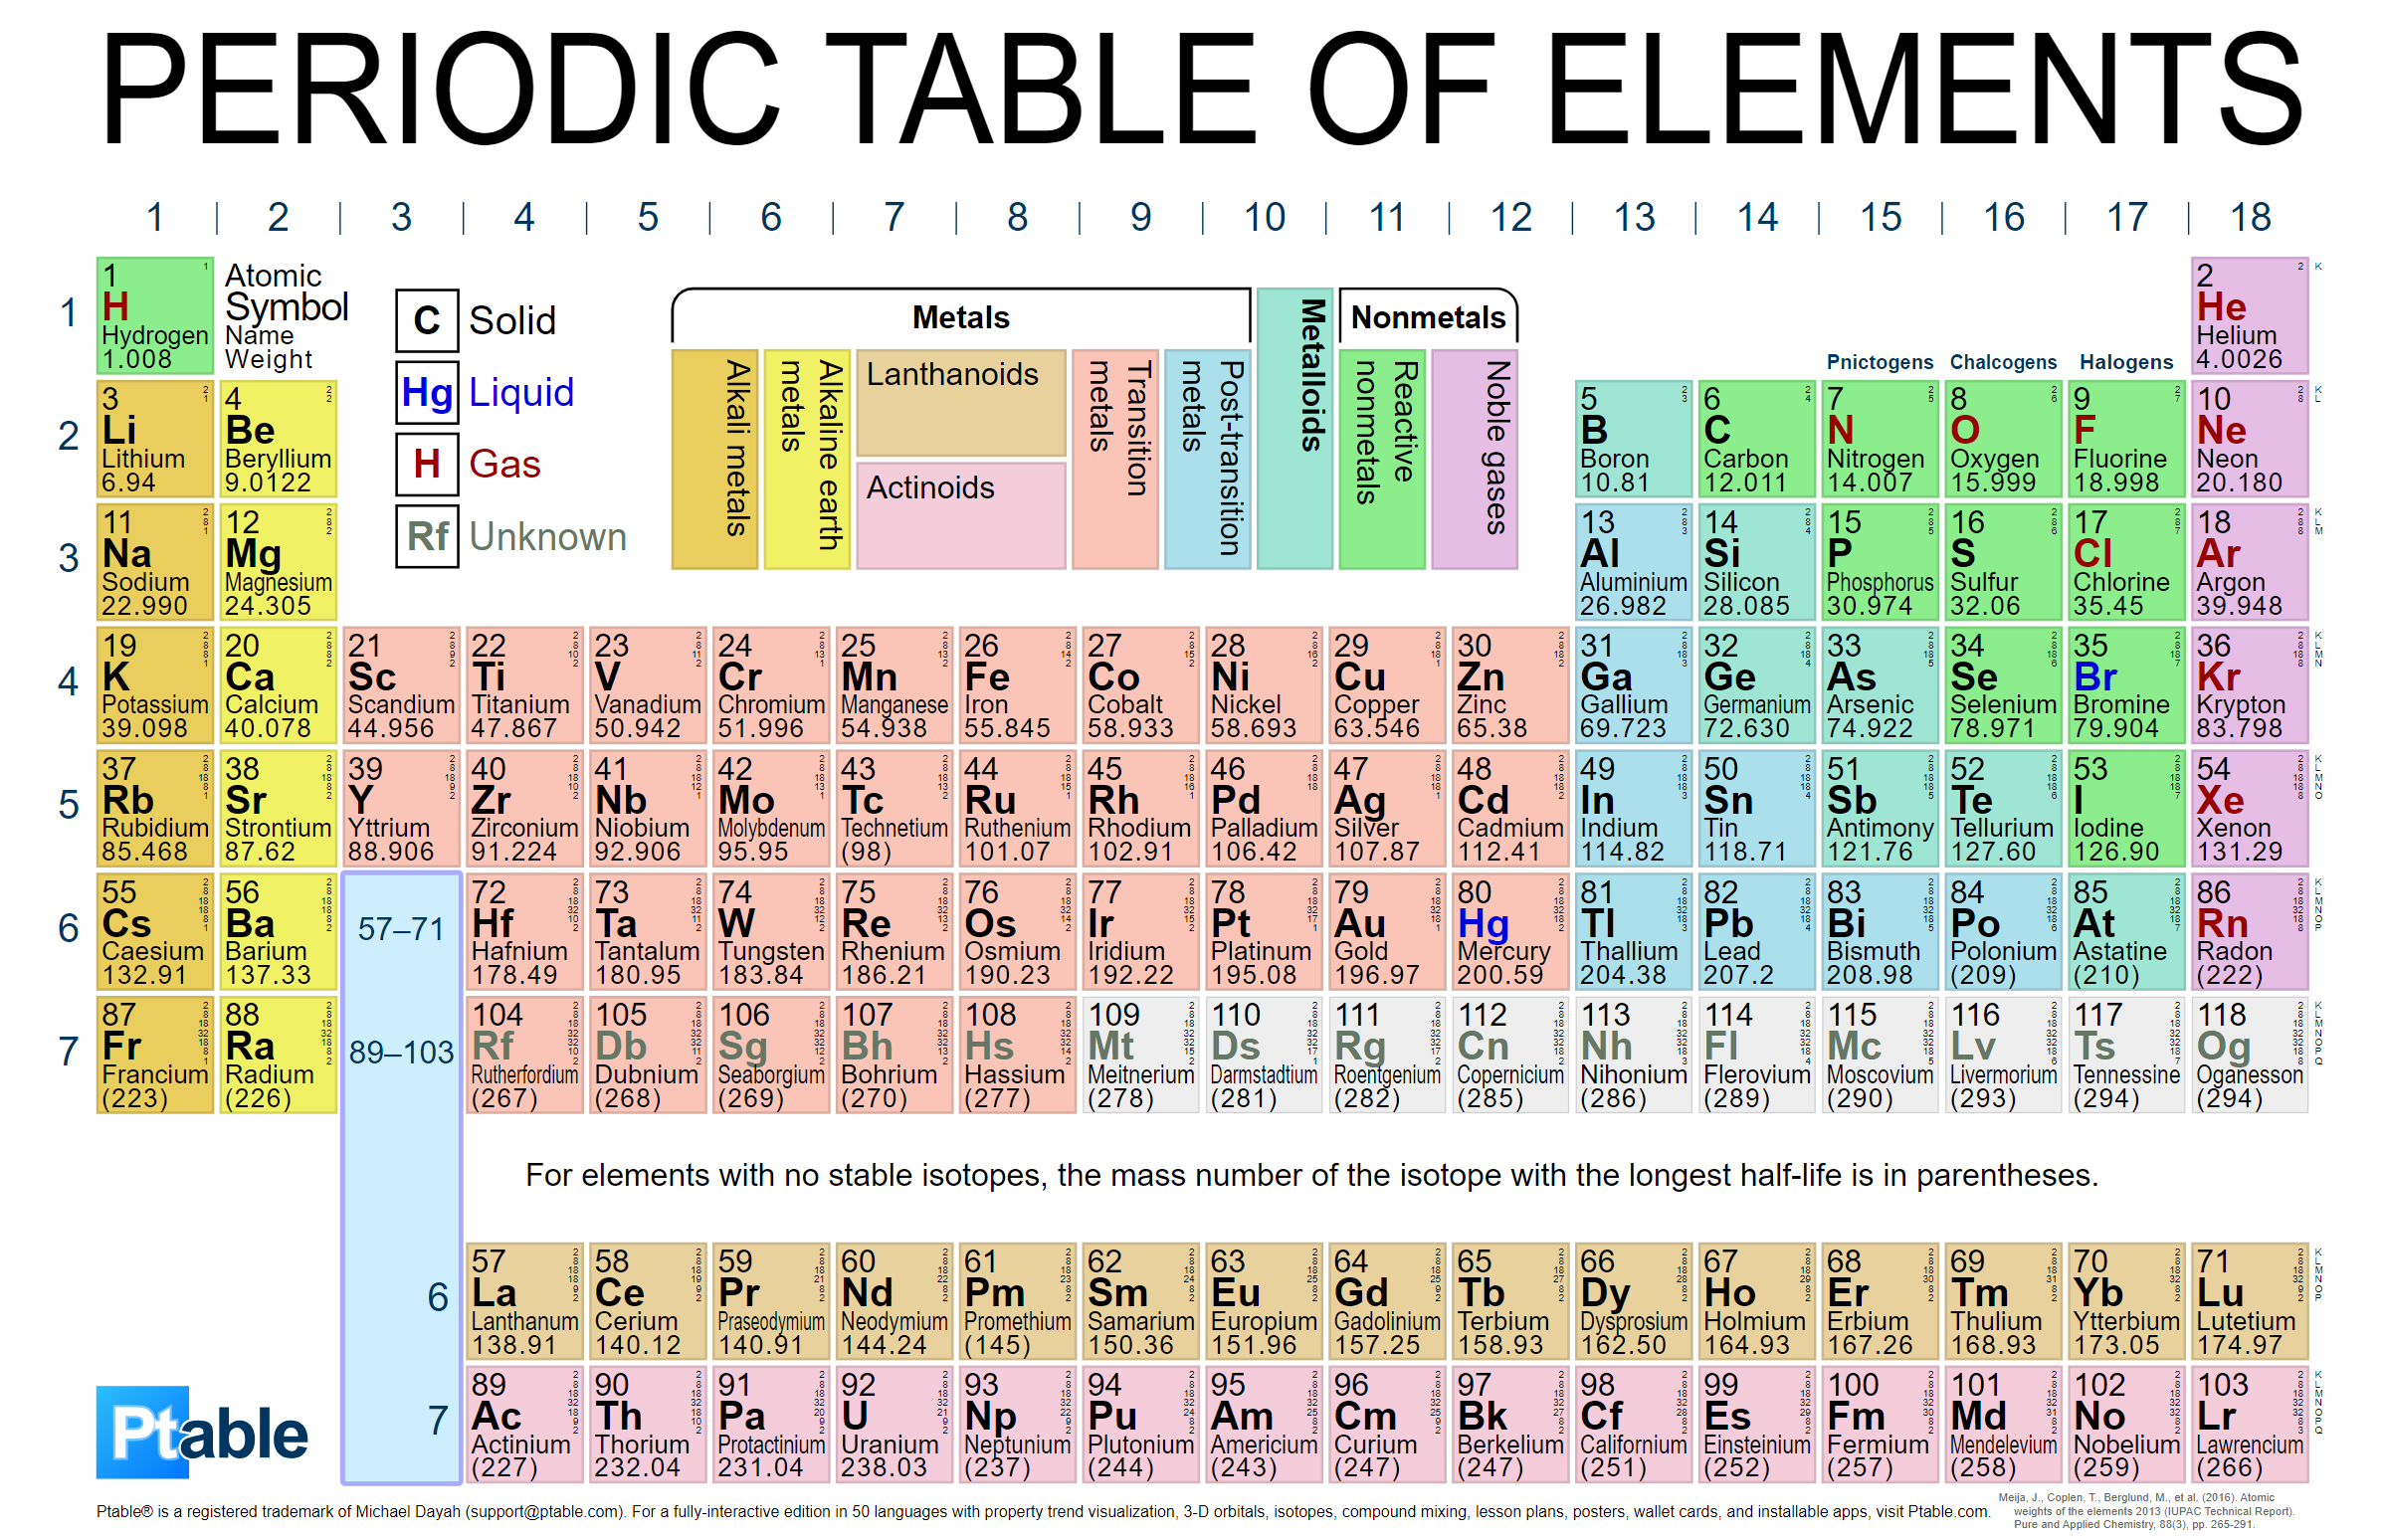
\includegraphics[angle=90,origin=c,width=.629\paperwidth]{img/periodic-table.png}}
    \caption{Periodiska systemet.}
\end{figure}
\vfill
\pagebreak

\section{Formelsamling}
\centering
\begin{table}[h!]
    \def\arraystretch{1.5}
    \centering
    \caption{Konstanter.}\vspace{5pt}
    \begin{tabular}{c | c | c}
        \textbf{Konstant} & \textbf{Symbol} & \textbf{Värde} \\ \midrule
        Pi & $\pi$ & \num{3.14159265359} \\
        Ljusets hastighet & $c$ & \SI{299792458}{\m\per\s} \\
        Wiens förskjutningskonstant & $b$ & \SI{2.8977719e-3}{\m\kelvin}
    \end{tabular}

\end{table}

\begin{table}[h!]
    \def\arraystretch{1.5}
    \centering
    \caption{Formler.}\vspace{5pt}
    \begin{tabular}{c | c}
        \textbf{Formel} & \textbf{Uttryck} \\ \midrule
        Wiens förskjutningslag & $\displaystyle \lambda_\text{max} = \frac{b}{T}$ \\
        Massa-energiekvivalens & $\displaystyle E = mc^2$
    \end{tabular}

\end{table}